\documentclass[10pt,a5paper]{article}
\usepackage[margin=1cm]{geometry}
\usepackage[utf8]{inputenc}
\usepackage[IL2]{fontenc}
\usepackage[czech]{babel}
\usepackage{microtype}
\usepackage{amssymb}
\usepackage{amsthm}
\usepackage{amsmath}
\usepackage{xcolor}
\usepackage{graphicx}

\usepackage[inline]{enumitem}

\newcommand{\hint}[1]{{\color{gray}\footnotesize\noindent(Nápověda: #1)}}

\setlist[enumerate]{label={(\alph*)},topsep=\smallskipamount,itemsep=\smallskipamount,parsep=0pt}
\setlist[itemize]{topsep=\smallskipamount,noitemsep}

\def\tisk{%
\newbox\shipouthackbox
\pdfpagewidth=2\pdfpagewidth
\let\oldshipout=\shipout
\def\shipout{\afterassignment\zdvojtmp \setbox\shipouthackbox=}%
\def\zdvojtmp{\aftergroup\zdvoj}%
\def\zdvoj{%
    \oldshipout\vbox{\hbox{%
        \copy\shipouthackbox
        \hskip\dimexpr .5\pdfpagewidth-\wd\shipouthackbox\relax
        \box\shipouthackbox
    }}%
}}%


\newtheorem*{poz}{Pozorování}

\theoremstyle{definition}
\newtheorem{uloha}{Úloha}
\newtheorem{suloha}[uloha]{\llap{$\star$ }Úloha}
\newtheorem*{bonus}{Bonus}
\newtheorem*{defn}{Definice}

\pagestyle{empty}

\let\ee\expandafter

\def\vysld{}
\let\printvysl\relax
\let\printalphvysl\relax

\makeatletter
\def\vyslplain#1{\ee\ee\ee\gdef\ee\ee\ee\vysld\ee\ee\ee{\ee\vysld\ee\printvysl\ee{\the\c@uloha}{#1}}}
\let\vysl\vyslplain

\def\locvysl#1{\ee\gdef\ee\locvysld\ee{\locvysld\item #1}}
\let\lv\locvysl

\newenvironment{ulohav}[1][]{\begin{uloha}[#1]\gdef\locvysld{\begin{enumerate*}}}{\ee\vyslplain\ee{\locvysld\end{enumerate*}}\end{uloha}}
\newenvironment{sulohav}[1][]{\begin{suloha}[#1]\gdef\locvysld{\begin{enumerate*}}}{\ee\vyslplain\ee{\locvysld\end{enumerate*}}\end{suloha}}

\makeatother

\begin{document}

\section*{Teorie grafů}


\begin{uloha}
Nalezněte isomorfismy mezi těmito grafy (jde o tzv. \emph{Petersenův graf}):
\[ 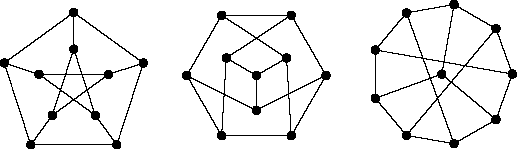
\includegraphics[width=10cm]{petersens.pdf} \]
\vysl{Např. 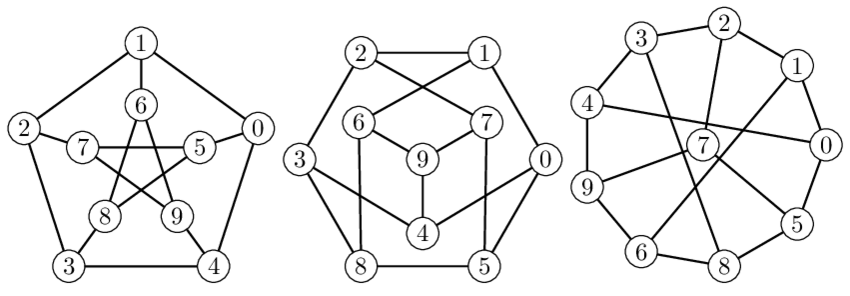
\includegraphics[width=10cm]{petersens_sol.png}}
\end{uloha}


\begin{ulohav}
Mějme tři vrcholy, $a$, $b$, $c$.
\begin{enumerate}
	\item Kolik existuje různých grafů na těchto třech vrcholech?\lv{8}
	\item Kolik jich je, pokud bereme isomorfní grafy za stejné?\lv{4}
\end{enumerate}
\end{ulohav}

\begin{uloha}
Nalezněte nějaké dva neisomorfní grafy na šesti vrcholech, které budou mít stejné skóre.
\vyslplain{Jedna možnost je vzít cestu na pěti vrcholech, ke které připojíme nový vrchol buď doprostřed, nebo do vrcholu sousedícího s prostředním.}
\end{uloha}

\begin{uloha}
Nalezněte všechny možné neisomorfní grafy se skóre $(3,3,3,3,3,3,6)$.
\vysl{Jsou dva: vrchol stupně šest musíme spojit se všemi ostatními, které budou tvořit buď cyklus délky šest, nebo dva \uv{trojúhelníky}.}
\end{uloha}

\begin{uloha}
Sestrojte co nejmenší příklad grafu s 6 vrcholy stupně 3, ostatními vrcholy stupně 2 a právě 12 hranami.
\vysl{Jedna možnost je vzít cyklus délky šest a každou druhou hranu rozšířit na \uv{trojúhelník}.}
\end{uloha}

\begin{uloha}
Rozhodněte, zda existuje graf na alespoň dvou vrcholech, jehož skóre by bylo tvořeno různými čísly. (Odpověď zdůvodněte.)
\vysl{Ne: stupeň může být max. počet vrcholů mínus jedna, takže \uv{aby se to vešlo}, musel by existovat jak vrchol tohoto max. stupně (který by byl spojen se všemi dalšími), tak vrchol stupně nula, což nemůže nastat současně.}
\end{uloha}

\begin{uloha}
Graf nazveme \emph{souvislý}, pokud se z každého vrcholu do každého umíme dostat po cestě z hran. Kolik hran může nanejvýš obsahovat nesouvislý graf s $n$ vrcholy? \vysl{$\frac{n(n-1)}{2} - (n-1)$}
\end{uloha}

\begin{suloha}
Dokažte, že má-li v grafu na $n$ vrcholech každý vrchol stupeň větší než $\frac n2$, tak už graf nutně obsahuje trojúhelník (tj. tři vrcholy, každý spojený s každým).
\end{suloha}

\medskip
\noindent
V následujícím se budeme zabývat \emph{stromy}, což jsou souvislé grafy bez cyklů.

\begin{uloha}
Rozmyslete si, že každý strom na alespoň 2 vrcholech má alespoň 2 vrcholy stupně 1 (tzv. \emph{listy}).
\end{uloha}

\begin{uloha}
Rozmyslete si, že každý strom má nutně o jedna méně hran, než má vrcholů. \hint{Podle předchozí úlohy musí na stromě existovat listy; postupně ten graf \uv{otrháme}.}
\end{uloha}

\begin{uloha}
Rozmyslete si, že každý souvislý graf, který má o jedna méně hran než vrcholů, je už nutně strom. \hint{Analogicky k předchozí úloze postupně otrháme graf.}
\end{uloha}


\newpage
\parindent=0pt
\parskip=\smallskipamount
\def\printvysl#1#2{\textbf{#1.}\ #2\par}
\vysld


\end{document}

